\documentclass[titlepage, a4paper, ngerman]{article}

\usepackage[utf8]{inputenc}
\usepackage[ngerman]{babel}
\usepackage{graphicx}

\author{Stefanie Gareis\\\texttt{stefaniegareis@mytum.de}}
\title{Falter, MATLAB und Simulink}
\date{\today}
%
%--------------------------------------------------------------------------
%
\begin{document}

\setcounter{secnumdepth}{2}
\maketitle
\pagenumbering{roman}
\tableofcontents
\newpage
\pagenumbering{arabic}
\setcounter{page}{1}
%
%--------------------------------------------------------------------------
%
%Simulink und das Modell
\part{Simulink, Modell und Simulation}
\rule{\linewidth}{0.5mm}
\setcounter{section}{0}
\section{Simulink}
Simulink ist ein recht umfangreiches Simulationsprogramm, bei dem ein Modell mit Blöcken aufgebaut wird. Ein großer Vorteil von Simulink ist die Möglichkeit VRML-Welten einzubinden (siehe auch Seite \pageref{vrml}), mit der man das zu simulierende Objekt auch grafisch darstellen kann.\\
Zusätzlich zu den von Simulink bereitgestellten Blöcken ist es auch möglich Matlab-Funktionen in das Diagramm einzubinden, um Funktionen bereitzustellen die Simulink nicht bietet.

\section{Aufbau des Modells}

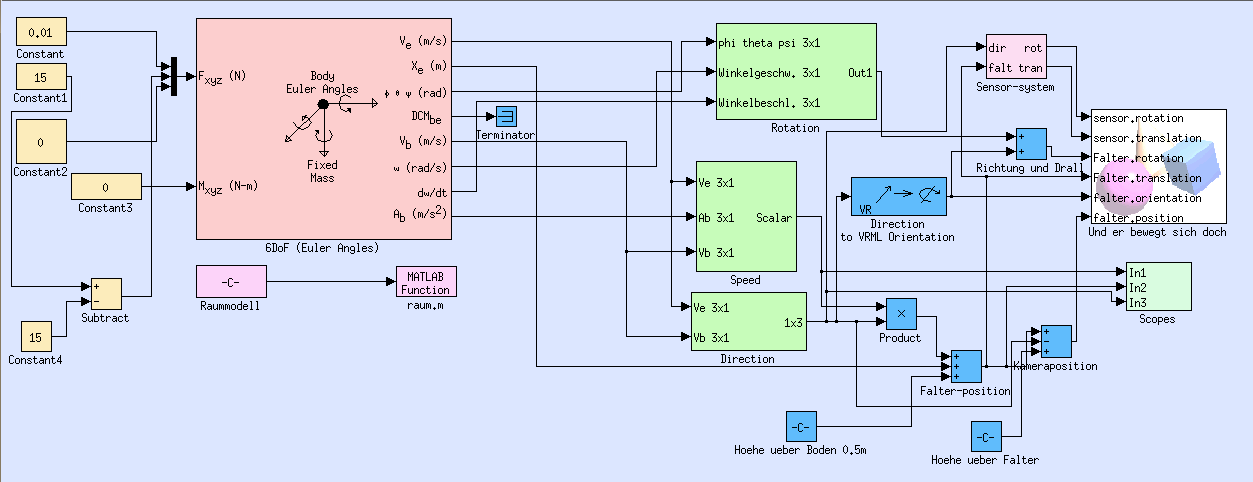
\includegraphics[width=\linewidth]{modell.png}
\\
Das Modell freedom.wrl besitzt vier \glqq Hauptblöcke\grqq \, für die Hauptarbeit der Simulation erledigen. Diese sind 6DoF (Euler Angles), Rotation, Speed und Direction.

\subsection{6 Degrees of Freedom (=6DoF) - Euler Angles}
Dieser Block erledigt alle aeronautischen Berechnungen, um aus wenigen Kräften Geschwindigkeit, Flug"-höhe, und Rotationen zu berechnen. Es gibt acht Aus"-gänge von denen für dieses Modell nur sechs notwendig sind.\\
$V_{e}$ und $V_{b}$ sind Geschwindigkeiten des Falters, einmal im Bezug zur Erde und einmal im Bezug zum Objekt; $X_{e}$ ist seine aktuelle Position. Aus diesen Daten lässt sich die Ortsveränderung (bezogen zum Ursprung) des Falters ermitteln.\\
$\Phi$, $\Theta$ und $\Psi$  sind die drei Eulerschen Winkel, die die Drehung um die Eigene Achse beschreiben, die Geschwindigkeit dieser Drehung wird mit $\omega$ beschreiben, ihre Beschleunigung mit d$\omega$/dt.

\subsection{Rotation}
Der {\em Rotation}--Block ist ein selbst erstelltes Subsystem, welches als Eingangsparameter die Eulerschen Winkel $\Phi$, $\Theta$ und $\Psi$\footnote{pitch, roll und yaw}, die Winkelgeschwindigkeit $\omega$ und die Winkelbeschleunigung $\omega$ besitzt.\\
Der Ausgangsvektor enthält die entsprechende Rotationsachse und die Größe des Winkels, um den gedreht wird, jedoch nicht mehr als Euler Winkel, sondern als VRML-Rotation, welche aus einer Drehachse und einem Drehwinkel besteht.

\subsection{Speed}
Das Subsystem {\em Speed} erhält als Eingangsparameter $V_e$ und $B_b$, aus diesen wird der Betrag der Geschwindigkeit berechnet, welche dann mit dem normierten Richtungsvektor multiplizeiert wird. Nimmt man die Beschleunigung $A_b$ hinzu, um die (evtl. physikalisch korrektere) Geschwindigkeit zu ermitteln, führt dies zu unerklärlichen Sprüngen des Modells, seine Geschwindigkeit bleibt jedoch gleich (es verändert sich also nichts), aus diesem Grund wurde sie rausgenommen.

\subsection{Direction}
Der Block {\em Direction} berechnet aus den Eingangsvektoren $V_e$ und $V_b$ einen Ausgangsvektor, der die normierte Richtung darstellt, diese Multipliziert mit der Geschwindigkeit ergibt die Ortsveränderung.

\section{Scope}
\label{scope}
Ein Scope ist ein Diagramm, welches eine beliebige Anzahl von Werten ohne großen Aufwand darstellen kann, die ist besonders gut, wenn man schnell mal ein paar Werte überprüfen möchte, ohne aufwändige Funktionsplots. Die Scope in dem Modell freedom.mdl zeigt momentan die Werte für Geschwindigkeit, Flughöhe und zurückgelegte Wegstrecke an. Unter dem Namen \glqq Scope 1\grqq \ ist es im Scope-Manager auffindbar und kann dort mit weiteren Parametern gefüttert werden.

\section{Plots}
\label{plots}
Ein weiterer wichtiger Teil zum Überwachen der Werte, sind die Funktionsplots. Diese werden in der Funktion {\em plotInstruments.m} erzeugt. Jeder dieser Plots besteht egtl aus zwei Funtkionen: Zum einen das Bild, das mit image(Bild) geplottet wird und zm anderen der Pfeil, der auf die Werte auf dem Bild zeigt.\\
Ein image()-Plot benötigt relativ viel Rechenzeit, weshalb die Plots nicht ständig erneuert werden, sondern erst alle 0.5-Simulations-Sekunden. Dieser Wert bietet eine gesunde Mischung zwischen flüssiger Anzeige und annehmbarer Simulationszeit.\\
Um einen neuen Plot hinzuzufügen, muss die Funktion {\em plotInstruments.m} ver"-än"-dert werden. Momentan werden pro Figure 6 Unterplots erzeugt, möchte man eine Funktion mehr, muss auch ein Plot mehr hinzugefügt werden; dies geschieht mit der Funktion subplot(x,y,i). Diese legt fest, wie die Plots angelegt werden, wie viele es sind und an welcher Stelle der jeweilige Plot liegt.\\
Um mehrere Plots übereinander darzustellen bietet es sich an ein \glqq hold on/off\grqq \ zu verwenden, alle veränderungen auf dem Plot nach einem \glqq hold on\grqq \ werden auf denselben Plot draufgelegt, bis zu einem \glqq hold off\grqq.

\section{Schnittstelle VRML-Simulink}
Die Schnittstelle zwischen VRML und Simulink ist der Block \glqq VR Sink\grqq \ . Mit diesem Block kann man einen VR-Viewer öffnen und dort die entsprechenden Block Parameter ändern. Hier kann man eine VRML-Welt (in diesem Fall walls.wrl) auswählen und ihre Knoten verändern, um die gewünschte Simulation zu erhalten.\\
Die Ausgänge der vorangegangenen Blöcke werden noch ein wenig verrechnet um korrekte Darstellungen zu liefern und landen dann in den Eingängen Falter.rotation, Falter.translation, falter.orientation und falter.position. Die kleingedruckten falter-Felder greifen auf die Kamera zu, die anderen direkt auf den Falter, auf dass er sich bewege und die Welt entdecke.
%
%----------------------------------------------------------------------------------
%
\newpage
%erklärt die Simulation
\part{Virtual Reality}
\rule{\linewidth}{0.5mm}
\setcounter{section}{0}
\section{VRML}
%aus section(simulink)
\label{vrml}
Die Virtual Reality Modelling Language (VRML) ist eine relativ alte Sprache, die zum Erstellen virtueller Welten dient. Zu Zeiten von Netscape erfreute sie sich großer Beliebtheit, da man sie leicht in HTML einbinden konnte und es auch entsprechende PlugIns für die damaligen Browser gab. Heute ist davon nicht mehr viel übrig, die VRML wird egtl. nur noch von Simulink verwendet und dient hier zur Visualisierung modellbasierter Systeme.

\subsection{Knoten (engl. Nodes)}
%aus Einführung subsection{Auf Knoten eine Welt zugreifen}
\label{nodes}
Jede VRML-Welt besteht aus mehreren Knoten. Diese bilden dann eine Welt, in walls.wrl ist ein solcher Knoten z.B. der Falter. Ein Knoten wiederum hat mehrere Felder, die die Eigenschaften des Knotens festlegen, der Falter hat z.B. die Felder {\em translation} und {\em rotation}.

\subsection{Prototypen}
%Referenz aus dem Einführungsteil hier hin
\label{protos}
Zusätzlich zu den Knoten gibt es auch Prototypen, diese sind vergleichbar mit den abstrakten Klassen in Java, sie selbst repräsentieren kein Objekt, jedoch ist es möglich mit ihnen vordefinierte Objekte zu erstellen. walls.wrl enthält 4 Sorten von Prototypen: {\em wall, ground, box} und {\em sphere}.\\
Ein neuer Protoyp erhält einen eigenen individuellen Namen und ist ab seiner Erzeugung auch als Knoten mit den definierten Eigenschaften verfügbar.

\subsubsection{wall, ground}
Wall und ground ermöglichen es Wände zu erzeugen, die entweder auf dem Boden liegen oder senkrecht stehen, schräge Wände zu erstellen ist noch nicht möglich. Wände und Böden haben die Felder \glqq position\grqq \ und \glqq size\grqq, diese legen fest wo sich der Mittelpunkt einer Wand befindet und wie sie gedreht ist.

\subsubsection{box, sphere} 
Box und Sphere dienen dazu Hindernisse in die Welt einzubauen, die der Falter selbstständig erkennen soll. Eine Box hat das Feld {\em position}, welches die Position der Box festlegt und {\em Size}, welches die Größe in den drei Dimensionen festlegt. \\
Eine Sphere besitzt ebenfalls eine {\em position} und außerdem einen {\em radius}, der den Radius festlegt, damit die Kugel in allen drei Richtungen dieselbe Ausdehnung hat, also nicht zu einer Ellipse deformiert werden kann.

\subsection{Viewpoints}
Für diese Welt stehen drei Blickpunkte (engl.: Viewpoints) zur Verfügung:
{\em here, falter} und {\em watch.}\\
Jeder dieser Blickpunkte ist spezifiziert durch eine Blickrichtung und eine Position und kann wie ein Knoten behandelt werden. Ein besonderer Blickpunkt ist {\em falter}, er verfolgt den Falter und hat ihn immer im Blick, als würde man hinter ihm her laufen.
%
%--------------------------------------------------------------------------------------
%
%Anleitung
\newpage
\part{Anleitungen}
\rule{\linewidth}{0.5mm}
\setcounter{section}{0}
\section{Die Welten}
Es befinden sich bereits einige fertige Welten in dem Ordner, die wichtigste ist walls.wrl. Eine VRML-Welt ist mit mehreren Knoten aufgebaut, jeder Knoten repräsentiert ein Objekt, walls.wrl enthält zusätzlich Prototypen, die wie Klassen funktionieren und mit denen sehr leicht neue Objekte angelegt werden können. Der einzige richtige Knoten in walls.wrl ist das Modell des Falters. Jeder Knoten besitzt einige Eigenschaften die ihn Näher Spezifizieren, beim Falter sind die wichtigsten {\em translation} und {\em rotation}, diese ermöglichen eine Verschiebung (= {\em translation}) und eine Rotation (= {\em rotation}) um den Mittelpunkt des Falters. \\
freedom.wrl ist eine fertige Welt, sie beinhaltet einen groben Plan des fortiss-Stockwerks und eine Heat-Map, die der Falter zur Orientierung erhält und welche sich während der Simulation ändern kann. finalgrid.wrl schließlich enthält diese Heat-Map und ist durch einen Inline-Befehl in freedom.wrl und walls.wrl eingebunden.

\subsection{Eine Welt zum bearbeiten öffnen}
Folgende Kommandos dienen zum öffnen und Bearbeiten einer Welt:
\begin{verbatim}
world = vrworld('VRML-world.wrl')
open(world);
view(world);
   -- Die Welt wird sichtbar gemacht
\end{verbatim}

\subsection{Auf Knoten in der Welt zugreifen}
Jeder Gegenstand in einer Welt wird durch einen Knoten (Seite \pageref{nodes}, Abschnitt \ref{nodes}) repräsentiert.
\begin{verbatim}
nodes(world); 
   -- zeigt alle diese Knoten an
fields(world.node) 
   -- zeigt alle veränderbaren Felder eines Knoten an, z.B. Position und Rotation
node = vrnode(world, 'node'); 	
   -- Legt einen Zeiger auf einen Knoten an
node = vrnode(world, 'node-Name', 'prototype');	
   -- legt einen neuen Knoten des Typs prototype an,
   -- Prototypen dienen der schnellen und einfachen Erzeugung von Objekten
world.node.field = ... 
   -- greift auf ein veränderbares Feld eines Knotens zu

\end{verbatim}

\section{Die Funktionen}
Da walls.wrl ohne Wände etwas leblos ist, gibt es einige Funktionen, die Objekte in dieser Welt erzeugen können entweder einzeln oder gleich mehrere.

\subsection{newWall.m}
Diese Funktion erzeugt über zwei verschiedene Prototypen (Seite \pageref{protos}, Abschnitt \ref{protos}) Wände und Boden, welches von beiden verwendet wird, entscheidet dabei die Funktion selbst. Um eine Wand zu erzeugen braucht es drei Vektoren, den Ortsvektor zu einem Eckpunkt der Wand und die zwei Vektoren die die Wand aufspannen, zusätzlich ist noch ein Index notwendig, da jede Wand einen eigenen Namen erhalten muss und dies durch einen Index am einfachsten zu realisieren ist, v. a. bei der automatischen Erzeugung.
Eine Wand erhält dann den Namen \verb|wall_index|.

\subsection{newBox.m, newSphere.m}
Diese Funktionen bieten die Möglichkeit Hindernisse in den Plan mit einzubinden, auch sie werden durch einen Positionsvektor bestimmt.\\ 
Die Größe der Box wird durch einen weiteren Vektor bestimmt, der ihre Ausdehnung in den drei Dimensionen beschreibt.\\
Die Größe der Kugel wird durch ihren Radius bestimmt.\\
Beide brauchen wiederum einen Index, der für einen individuellen Namen steht (entspr. \verb|box_index| , \verb|sphere_index|).

\subsection{raum.m, raum.mat, deleteWalls.m getObjects.m}
In raum.m wird eine Matrix übergeben, die eine ganze Liste von Wänden enthält, diese werden dann automatisch an newWall.m übergeben und somit wird ein Raum erzeugt, der aus den Wänden \verb|wall_0 - wall_matrix-height| besteht.\footnote{Raum.mat enthält eine solche Matrix, mit der ein grober Plan des fortiss-Stockwerkes erzeugt werden kann.}\\
DeleteWalls.m löscht alle Wände der Welt, die übergeben wird.\\
GetObjects hat drei Rückgabeparameter: walls, boxes und spheres, mit
\begin{verbatim}
[walls, boxes, spheres] = getObjects(world)
\end{verbatim}
bekommt man drei Matrizen, \verb|walls| gibt eine Karte zurück, mit welcher auch wieder ein Raum erzeugt werden kann, \verb|boxes| und \verb|spheres| geben die jeweiligen Positionen und Größen der Hindernisse an.

\subsection{mygrid.m}
Die Heat-Map, welche der Falter während seines Fluges erzeugt besteht aus Wahrscheinlichkeitswerten zwischen 0 und 255, die die Wahrscheinlichkeit eines Hindernisses angeben. Diese Heat-Map kann 3-dimensional dargestellt werden, und auch farblich hervorgehoben werden.\\
Die Darstellung und Einfärbung erfolgt mit der Funktion mygrid.m welche ein VRML-Dokument erzeugt, das dann mit einem \verb|Inline|-Befehl\footnote{Inline \{ URL "'finalgrid.wrl"' \}}  in eine beliebige Welt eingebunden werden kann. \\
mygrid.m kann verschiedene Aufgaben zusätzlich zum Anlegen der Map erledigen, diese können direkt nach Bedarf ein- oder auskommentiert werden. 
Um Zeit zu sparen kann die Einfärbung weggelassen werden, dazu einfach die Zeilen 43-63 mit \glq\%\grq auskommentieren und in Zeile 45 statt \verb| color Color|, \verb| color NULL| einfügen. Es kann auch eine Textur statt einer Färbung verwendet werden, dazu im oberen Teil, diese Zeilen ein kommentieren. Wem das Gitter zu solide ist, der kann auch die Zeilen 36 - 41 hinzunehmen, diese sorgen dafür, dass nicht das gesamte Gitter 3D ist, sondern nur ca. die Hälfte der Pixel aus dem Boden heraus sticht.

\section{Das Simulink Modell}
Der Simulink-Teil des ganzen befindet sich vollständig in freedom.mdl. In diesem Modell wird walls.wrl als Standardwelt verwendet, erst während der Simulation werden hier Wände eingefügt. Es ist auch möglich während der Simulation die Heat-Map erzeugen zu lassen, jedoch muss man auf die Größe der Heat-Map achten, da diese die Simulationszeit stark verlangsamen kann, alternativ kann man auch die Refresh-Time der Funktion mygrid.m vergrößern, sodass die aufwändige Berechnung nicht mehr sooft stattfinden muss.

\subsection{Fliegen lassen}
Wenn man die Simulation startet, sollte sich der Falter in einem Viewer bewegen.\footnote{Doppelklick auf Simulationsblock öffnet einen Viewer} Es stehen drei Viewpoints zur Auswahl: {\em falter, here} und {\em watch.}\\
Der Viewpoint {\em falter} verfolgt alle Bewegungen des Falters und fliegt ihm auch nach, der Viewpoint {\em here} \ zeigt einen Schrägblich auf den gesamten Raum, schöner ist er, wenn man sich hier nur das Mesh anschaut (=kleinen Button mit Quader drauf drücken). Der Viewpoint {\em watch} betrachtet die Szenerie von oben, so dass man alle Bewegungen des Falters von oben beobachten kann.\\
Die 4 Konstanten oben links in dem Modell sind die Kräfte die auf den Falter wirken, diese können je nach belieben eingestellt werden, und der Falter bewegt sich in Richtung der entsprechenden Achse.

\subsection{Das Modell verändern}
Möchte man den Falter in einer anderen Umgebung fliegen lassen, kann man in einem VRML-Viewer in dem Menüpunkt Simulation, Block Parameters eine andere Welt wählen. Hier hat man auch die Möglichkeit festzulegen, auf welche Parameter das Modell zugreifen kann, dies geschieht wieder nach dem Knoten-System der VRML.\\
Sämtliche vorher vorgestellten Matlab-Funktionen lassen sich auch in Simulink einbinden mit dem Block \glqq Matlab Fcn\grqq. Daher kann man recht einfach die Erzeugung eines Raumes oder einer Heat-Map zur Laufzeit erledigen, was es ermöglicht auch kurzfristige Änderungen vorzunehmen.\\
Einen anderen Raum erhält man durch Veränderung der Konstante Raummodell. Diese beinhaltet eine Matrix, die in jeder Zeile eine Wand des Raumes darstellt.

\subsection{Die Anzeigen}
Um die Werte des Falters zu überwachen gibt es mehrere Anzeigen. \\
Geschwindigkeit, Flughöhe und zurückgelegte Strecke werden in einem {\em Scope} dargestellt  (siehe S. \pageref{scope}, Abschnit \ref{scope}). Hier kann man beliebige Signale mit aufnehmen, indem man sie der Signal-Liste hinzufügt, oder mit einem Rechts-Klick auf das entsprechende Signal zur gewünschten Scope hinzufügt. \\
Batterieanzeige, Flugwinkel, Geschwindigkeit, Flughöhe, Radar und ein Kompass werden durch Plots dargestellt (sh. S. \pageref{plots} Abschnitt \ref{plots}), die mit einer Matlab-Funktion aufgerufen werden.
{\bf WICHTIG:} Damit die Plots korrekt dargestellt werden und sich auch während der Simulation verändern können, muss ein Scope-Viewer geöffnet sein.\\
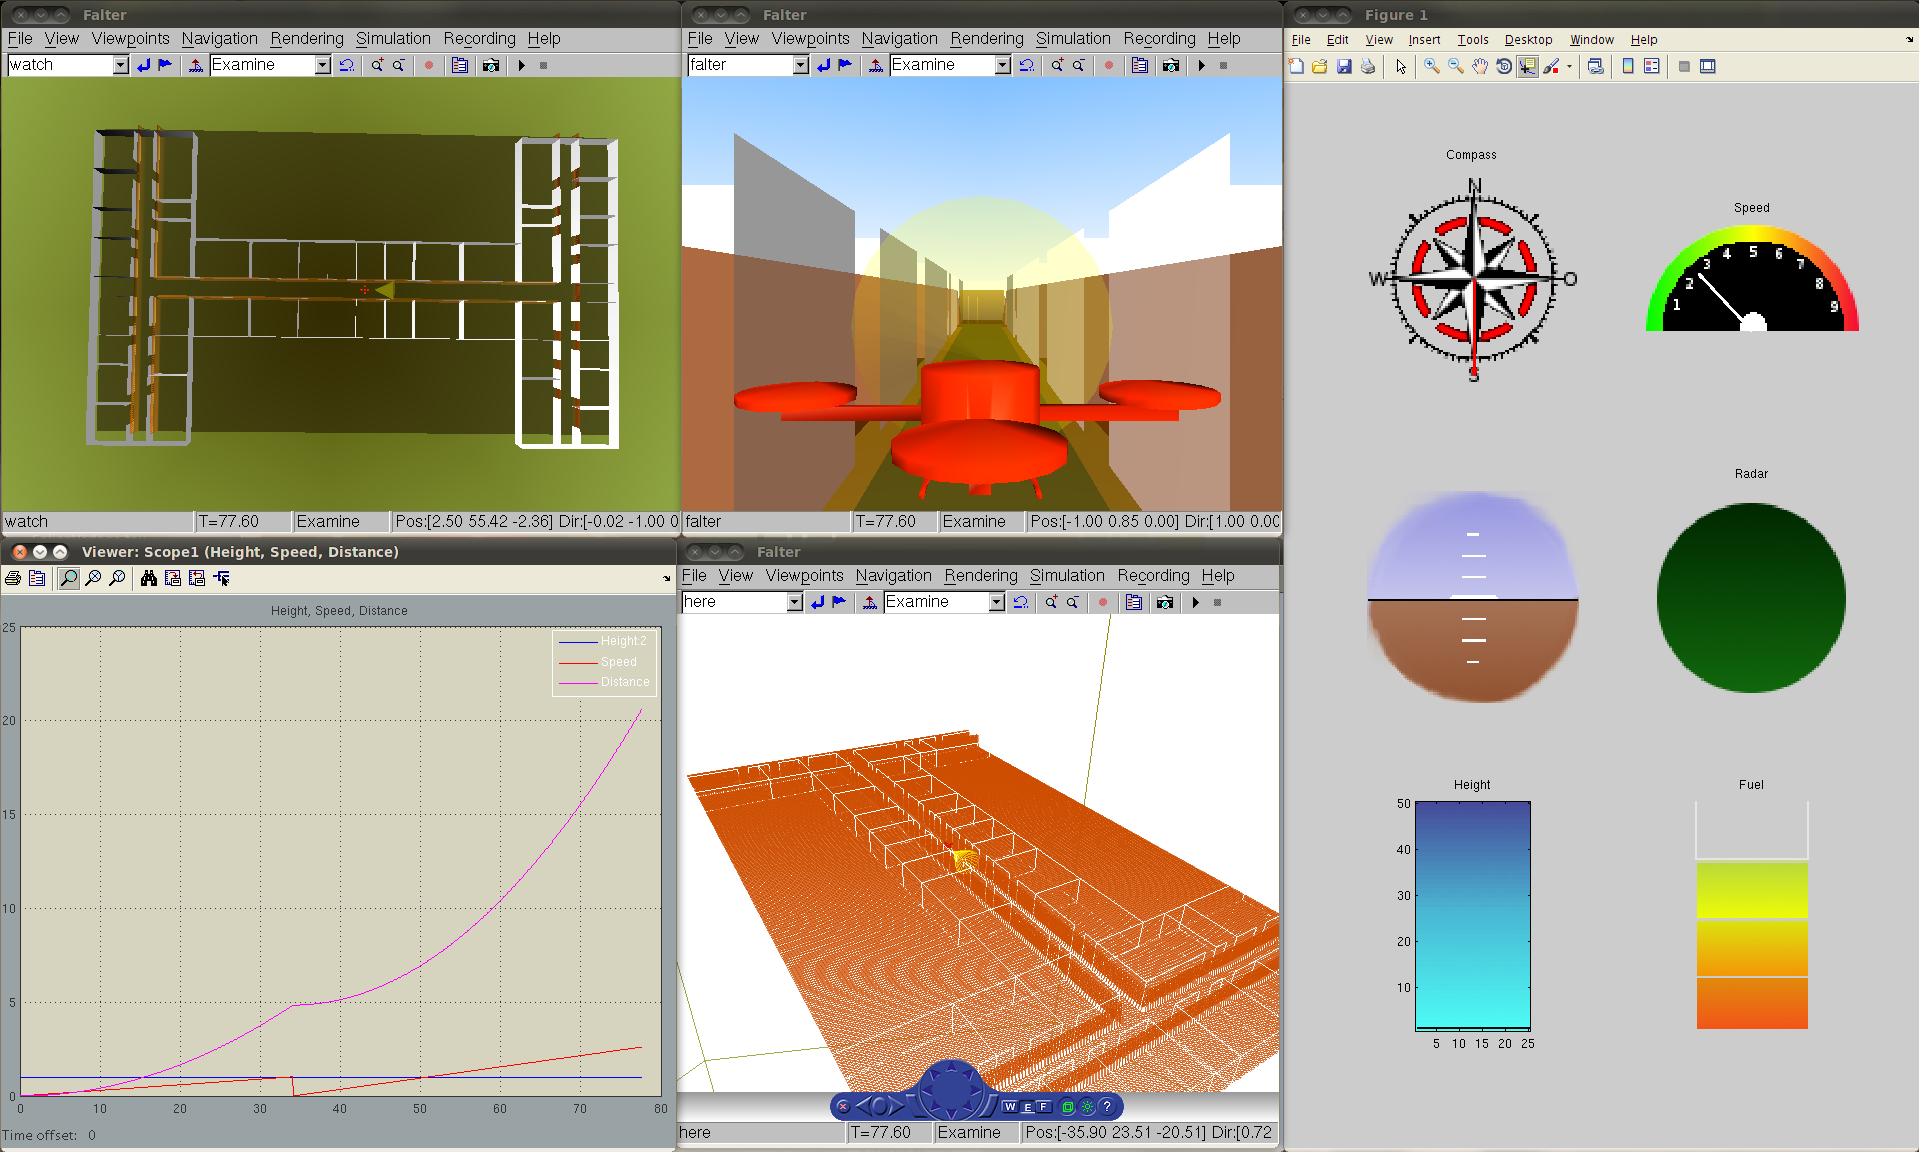
\includegraphics[width=\linewidth]{Bildschirmfoto.png}
%
%--------------------------------------------------------------------------------------
%
\newpage
%Anhang
\setcounter{secnumdepth}{1}
\appendix
\section{kleine Bugs und Fehler}
Fehler passieren immer und manche sind nur schwer zu beheben, weshalb hier mal die wichtigsten aufgeführt werden.
\subsection{Der Flug gen Osten}
Aus irgendeinem Grund wird alles auf den Kopf gestellt, wenn die Flugrichtung nur entlang der Positiven z-Achse erfolgt, sobald auch nur eine minimale Abweichung in eine andere Richtung auftritt, ist alles wieder in Ordnung.
\subsection{Der Sensor-Kegel}
Da Rotationen ein recht kompliziertes Thema in VRML sind, zeigen die Sesoren immer parallel zum Boden in die Flugrichtung, wenn man also nach oben fliegt, zeigt der Zylinder geradeaus, statt in Flugrichtung nach oben.
\subsection{Falter als Lichtquelle}
Der Falter scheint die Lichtquellen in hohem Maße zu beeinflussen, daher scheinen die Wände manchmal zu blinken, ist der Falter minimal durchsichtig, tritt dieses Problem nicht mehr auf.
\subsection{wall und ground}
Ebenfalls wegen der Rotation gibt es Probleme mit schrägen Wänden. Diese können nur gerade stehend oder flach liegend erzeugt werden.
\subsection{Physikalische Korrektheit}
Ich kann nicht garantieren, dass die Simulation alle Erfordernisse der Physik beachtet, womöglich sind einige der Angaben falsch bzw. verfälscht.\\
Manche Werte wurden auch ungefähr korrigiert, weshalb sie vermutlich nicht ganz korrekt sind, so zB die Distanz-Anzeige in der Scope. Dieser Wert stimmte nie mit irgendwas überein, einzig seine Berechnung ist korrekt. Um einen scheinbar genaueren Wert zu erreichen wird er durch 1.8($= 0.5 * 3.6$ Umrechnungsfaktor m/s zu km/h)  geteilt, aber ob die Abweichung linear oder oder sonstwie ist weiß ich nicht.\\
Beschleunigungs und Bremsverhalten wirken ebenfalls korrekt, da aber die Beschleunigungswerte nicht berücksichtigt werden, kann ich keine Garantie für Korrektheit abgeben, auch wenn die Beschleunigungswerte die Simulation scheinbar nicht ändern.

\end{document}
